\documentclass{article}

% ready for submission
\usepackage[final]{neurips_2021}
\usepackage[utf8]{inputenc} % allow utf-8 input
\usepackage[T1]{fontenc}    % use 8-bit T1 fonts
\usepackage{hyperref}       % hyperlinks
\usepackage{url}            % simple URL typesetting
\usepackage{booktabs}       % professional-quality tables
\usepackage{amsfonts}       % blackboard math symbols
\usepackage{nicefrac}       % compact symbols for 1/2, etc.
\usepackage{microtype}      % microtypography
\usepackage{xcolor}         % colors
\usepackage{algorithm2e}
\usepackage{amsmath}
\usepackage{graphicx}
\usepackage{float}
\usepackage{caption}
\usepackage{subcaption}

\usepackage[backend=biber, style=alphabetic, sorting=ynt]{biblatex}

\addbibresource{ref.bib}

\title{CS271 Project: Sokoban Solver}

\author{
  Seokchan Ahn\\
  15288114 \\
  \texttt{seokchaa@uci.edu} \\
   \And
  Youngil Kim\\
  87561931\\
  \texttt{youngik2@uci.edu}\\
   \And
  Jinhwa Kim \\
  86727408 \\
  \texttt{jinhwak@uci.edu}
}
\begin{document}

\maketitle

\begin{abstract}
  Sokoban is a game in which the player pushes boxes around in a warehouse, trying to get them to storage locations. Since the number of possible states can grow exponentially as the board size and number of boxes increase, we suggests model-free reinforcement learning(RL) based solver for this game. Among a variety of RL algorithms, we focus on Monte-Carlo(MC), Temporal-Difference(TD) and Q-learning, which are the most widely used methods.
\end{abstract}

\section{Sokoban}
Sokoban is a game that the user pushes the boxes to the proper storage locations with a minimum number of moves. The map is consists of floor, wall, boxes, and marked storage locations and the above figure shows an example of a state in the Sokoban game. The user can move in 4 directions: Up, Down, Left, Right, and it is not allowed to move through walls or boxes. There are two conditions for terminating the games: 1) All the boxes are on the goals. 2) Deadlocks.

\section{Algorithms}

We suggest three model-free RL algorithms to solve the problems. First two are the Monte Carlo and the Temporal Difference learning, which is a sampling-based prediction algorithms. The last one is Q-learning, which is a control algorithm using TD error.

Each of these algorithms may have different time complexities, but the space complexity would be all the same because all of them shares the same state space. The space complexity would be $O((MN)^{B+1})$ because ignoring the walls, there are $MN$ positions we can place a box or a player, and there are $B$ boxes and 1 player. However, we can save the space a lot in practice by pruning branches that never able to reach a goal.

\subsection{Monte Carlo (MC) Learning}
Monte Carlo Learning method is a way to solve the Reinforcement Learning problem by averaging sample returns. It is a model-free method which means this algorithm does not have knowledge of MDP transition. MC generates episodes and learns from them, but all episodes must terminate.


\RestyleAlgo{ruled}
\SetKwComment{Comment}{/* }{ */}
\begin{algorithm}[H]
\caption{Monte Carlo Learning}\label{alg:mc}
\KwData{State $s \in S$ , Action $a \in A(s)= \{U,D,R,L\}$}
Randomly initialize $Q(s,a)$ \;
Initialize $Returns(s,a) \gets empty list$\;
Initialize $\pi \gets random policy$\; 
\While{not policyChanged()}{
$episodes \gets generateEpisode(\pi) $\Comment*[r]{generate Episode sample}
\For {each pair $s,a$ in episodes}
{
 Append return of the first occurence of $s,a$ to $R(s,a)$\;
 $Q(s,a) \gets average(R(s,a))$\Comment*[r]{average reward of each episode}
}
\For{each $s$ in the episodes}
{
$a* \gets \underset{a}{\arg\max} Q(s,a) $\;
\For{all $a \in  A(s)$}
{
$\pi(s,a) \gets \epsilon-soft$ policy update \Comment*[r]{update Policy}
}
}
}
\end{algorithm}

\RestyleAlgo{ruled}
\begin{algorithm}[H]
\caption{Function generateEpisode()}\label{alg:genEpisode}
\KwData{$\pi,numberOfEpisodes$}
$episodes \gets $empty list\;
\While{ $n < numberOfEpisodes$}{
$timestamp \gets$ empty list\;
\While{not goalSate()}{
$ s, a ,r \gets getSAR(\pi)$\Comment*[r]{get State and Action from policy}
Append $ s, a ,r$ to $timestamp$\;
}
Append $timestamp$ to $episodes$\Comment*[r]{append the generated episode}
$n \gets n+1$ \Comment*[r]{increase number of step by 1}
}
\end{algorithm}

\textit{Policy Evaluation}
The Monte Carlo Learning method does not have a model. Thus, this model uses the mean return value of samples for evaluating policy instead of the expected return as Bellman expectation backup does. 

\textit{Problem on MC Learning}
Because MC learning initializes policy randomly, it could take infinite time to make a terminate episode. Thus, We can use Temporal Difference(TD) learning instead or update policy on the partial completed state, not on the completely ended state.

\textit{Time Complexity}
One step for the MC learning is generating a episode, averaging reward, and updating the policy. The max length of the episode is $MN$ where $M$ and $N$ denotes the board’s width and height. It means it iterates a loop at most $MN$ times for generating a episode and, therefore, the time complexity of one step would be $O(MN)$. If MC iterates $T$ steps to converge, the final time complexity of MC would be $O(MNT)$. 

\subsection{Temporal Difference(TD) Learning}
Temporal Difference is also one of model-free reinforcement learning methods, but most difference from MC methods comes from the fact that it does not necessarily require complete episodes, so it takes advantage of MC methods and Dynamic Programming (DP) methods by bootstrapping from the current estimate of the value function. In TD learning, the algorithm samples from the environment like MC methods, but performs updates based on current estimates like DP methods.

In TD Learning, we should consider 4 hyperparams; $\gamma$, $\lambda$, $\alpha$, and $\delta$. $\gamma$ is the discount rate, which is a value between 0 and 1. The higher the value the less you are discounting.  $\lambda$ is the credit assignment variable, which is also a value between 0 and 1. The higher the value the more credit you are able to assign to further back states and actions. $\alpha$ is the learning rate, showing how much of the error should we accept and adjust our estimates towards. Lastly, $\delta$ is a change in value. In our approach, we are planning to choose $\lambda$ is 0 for simplicity and efficiency.

\RestyleAlgo{ruled}
\SetKwComment{Comment}{/* }{ */}
\begin{algorithm}[H]
\caption{TD(0) Learning}\label{alg:td}
\KwData{the policy $\pi$ to be evaluated}
 Initialize $V(s)$\;
 \For{each episode}{
  Initialize $s$\;
  Initialize $step, maxStep$\;
  \While{$step \leq maxStep$}{
    $A \gets getAction(\pi, S)$ \Comment*[r]{get Action from policy $\pi$}
    $V(S) \gets V(S)+\alpha[R+\gamma V(S') - V(S)]$ \Comment*[r]{update $V(S)$}
    $S \gets S'$\Comment*[r]{update current state}
    \If{$isGoalState(s')$} {
      break\Comment*[r]{arrived to one of the goal states}
    }
    $step \gets step + 1$\Comment*[r]{increase current step by 1}
  }
 }
\end{algorithm}

The time complexity of TD(0) methods is $O(MNB)$ for each episode, where $M$ is width of the level, $N$ is height of the level, and $B$ is the number of the box in the level.

\subsection{Q-Learning}

Q-learning is a model-free reinforcement learning algorithm to learn the value of an action in a particular state. It is an off-policy learning because the executed actions are different from the target actions that are used for learning. It updates values based on the next state's best action, but choose the action by $\epsilon$-greedy policy, which enables both exploration and exploitation.

\begin{algorithm}[H]
\caption{Q-Learning}\label{alg:one}
\KwData{State $s \in S$ , Action $a \in A(s)= \{U,D,R,L\}$}
Initialize $Q(S, A)$ as zero\;
Initialize $maxStep, \epsilon, \alpha, \gamma$\;
Initialize $s$ \Comment*[r]{initial state}
$step \gets 1$\;

\While{$step \leq maxStep$}{
  $a \gets getAction(s, \epsilon)$ \Comment*[r]{choose action using $\epsilon$-greedy policy}
  $s', r \gets getNextState(action)$ \Comment*[r]{next state, reward}
  $Q(s, a) \gets Q(s, a) + \alpha(r + \gamma \max Q(S', a) - Q(s, a))$ \Comment*[r]{update Q for s, a}
  $s \gets s'$ \Comment*[r]{update state to new state}

  \If{$isTerminal(s')$)} {
    Initialize $s$ \Comment*[r]{start over from the initial state}
  }
  $step \gets step + 1$\Comment*[r]{increase current step by 1}
}
\end{algorithm}

We use $maxStep$ as an upper-bound of the length of each episode. Though Q-learning can learn without limiting the number of steps, having an upper-bound can make the learning process more efficient by preventing exploring the states far from the goal too much. This value must be greater than the length of the episode with the optimal solution since otherwise it will never reach to the goal state. Therefore, we use $maxStep$ of $MNB$ where $M$ and $N$ denotes the board's width and height, and $B$ denotes the number of boxes, since the maximum number of steps to move one box to the storage must be less than $MN$ and there are $B$ such boxes. As a result, the time complexity of this algorithm would be $O(MNB)$ for each episode and total training time would be in proportion to the number of iterations until the Q-values converge.

There are three hyper-parameters in Q-learning. First, $\epsilon$ decides the possibility of exploitation. In general, $\epsilon$ is initialized as a value close to 1.0, which means the agent will choose an action almost randomly, since there is no information about the expected value in the beginning. As the estimated Q-values converge, $\epsilon$ should be decayed to exploit the learned values. $\alpha$ and $\gamma$ are the learning rate and the discount rate by time for each.  

\begin{algorithm}[H]
\caption{Q-Learning Inference}\label{alg:two}
\KwData{State $s \in S$ , Action $a \in A(s)= \{U,D,R,L\}$}
Initialize $s$ \Comment*[r]{initial state}
$\epsilon \gets 0.0$ \Comment*[r]{greedy policy}

\While{$True$}{
  $a \gets getAction(s, \epsilon)$ \Comment*[r]{choose action using $\epsilon$-greedy policy}
  $s', r \gets getNextState(action)$ \Comment*[r]{next state, reward}
  $s \gets s'$ \Comment*[r]{update state to new state}
  \If{$isGoalState(s')$} {
    break \Comment*[r]{Arrived to one of the goal states}
  }
}
\end{algorithm}

In the inference time, the agent can greedy choose the best action at the current state every time. It can be done by simply using the $\epsilon$ value of zero. The time complexity would be $O(L)$ where $L$ denotes the length of the episode it generates and $L$ would be less than $M*N*B$.

\section{Implementation Details}

\subsection{States and Actions}

In the Sokoban game, states can be defined as the setting of the board. Since the positions of walls and the positions of storage are fixed, we can use the coordinations of the boxes and the player as a state. Since the order of boxes doesn't matter, we use a hash map for Q-table using $(set(boxes), player)$ as keys and Q-values as values. For actions, we use $[L, U, R, D]$ since they are all the available movements.

A Sokoban game's terminal states are 1) when all the boxes are on the storage or 2) when on a Deadlock state. In training time, we stop and re-initialize the state once the player reaches to a terminal state since we do not need to explore further. In inference time, we just stop and return the generated episode and its length.

\subsubsection{Deadlocks}

In Sokoban games, there is a state, which is called a deadlock, when an agent cannot reach any goal state, no matter what the agent moves. The only way to solve this problem is backtracking to the previous state or restarting the game. In order to solve the Sokoban game efficiently, it is inevitable to handle deadlocks properly. In this session, we will discuss a few types of deadlocks present in the Sokoban game, and will include some of them to our final result.
\footnote{http://sokobano.de/wiki/index.php?title=Deadlocks}

\paragraph{Simple deadlocks}
A simple deadlock is created by moving just one box to border lines, which makes it unable to reach any goal state, no matter what the agent moves. In the figure \ref{fig:simple}, pushing the box to a darker shaded space results in a simple deadlock.

\paragraph{Freeze deadlocks}
Freeze deadlocks refer to the situation that one of boxes becomes immovable. If a box becomes immovable while not being located on a goal, the game is deadlocked. In the figure \ref{fig:freeze}, pushing the box one square up results in a freeze deadlock.

\paragraph{Corral deadlocks}
Corral indicates a zone that the agent cannot access. Corral deadlocks can be created when deadlock happens if the agent is not able to move the box because of presence of corral. In the figure \ref{fig:corral}, marked area with little blue quadrats is a corral, and it is not reachable for the agent. Pushing the lower box to the right square results in a corral deadlock.

\begin{figure}
     \centering
     \begin{subfigure}[b]{0.3\textwidth}
         \centering
         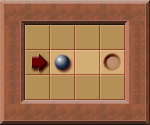
\includegraphics[width=\textwidth]{SimpleDeadlockExample.png}
         \caption{Simple Deadlock}
         \label{fig:simple}
     \end{subfigure}
     \hfill
     \begin{subfigure}[b]{0.3\textwidth}
         \centering
         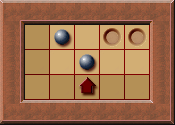
\includegraphics[width=\textwidth]{FreezeDeadlockExample.png}
         \caption{Freeze Deadlock}
         \label{fig:freeze}
     \end{subfigure}
     \hfill
     \begin{subfigure}[b]{0.3\textwidth}
         \centering
         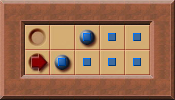
\includegraphics[width=\textwidth]{CorralDeadlockExample.png}
         \caption{Corral Deadlock}
         \label{fig:corral}
     \end{subfigure}
        \caption{Three simple graphs}
        \label{fig:deadlocks}
\end{figure}

\subsection{Rewards}
Rewards are the most important part in reinforcement learning since it decides which actions are good or bad and how good or bad they are. We defined the categories of rewards as below.

% Please add the following required packages to your document preamble:

\begin{table}[H]
\centering
\resizebox{\textwidth}{!}{%
\begin{tabular}{|l|l|p{8cm}|}
\hline
Category          & Reward & Description                                                                                                                         \\ \hline
MOVE              & -0.1   & To prevent looping infinitely, give small penalty for each move                                                                     \\ \hline
BOX\_ON\_STORAGE &
  1.0 &
  Since it may takes too many steps to the final goal, updating Q-values from the final reward is difficult. Therefore, giving rewards for achieving intermediate goals can make the Q converge faster. \\ \hline
BOX\_OFF\_STORAGE & -1.0   & Give penalty for pushing a box away from a storage.                                                                                 \\ \hline
ALL\_ON\_STORAGE  & 10.0   & Give reward when the player successfully finishes the game.                                                                         \\ \hline
DEADLOCK          & -10.0  & Once it gets to a deadlock state, it can never be solved afterwards. Therefore, give a great penalty and initialize the state again. \\ \hline
MOVE\_TO\_WALL    & -1.0   & Trying to go toward a wall or a box in front of another box or a wall is not worth. Therefore, give a small penalty.                \\ \hline
\end{tabular}%
}
\caption{Categories of rewards and their values}
\label{tab:rewards}
\end{table}


% \appendix

% \section{Appendix}

% Optionally include extra information (complete proofs, additional experiments and plots) in the appendix.
% This section will often be part of the supplemental material.

% \printbibliography

\section{References}

[1] Russell, S. J., Norvig, P., \& Davis, E. (2010). Artificial intelligence: a modern approach. 4th ed. Upper Saddle River, NJ: Prentice Hall.

% [2] Ketan Doshi. (2020). Reinforcement Learning Explained Visually (Part 4): Q Learning, step-by-step. Towards Data Science. https://towardsdatascience.com/reinforcement-learning-explained-visually-part-4-q-learning-step-by-step-b65efb731d3e

\end{document}